% !TEX root = tracking.tex
\section{Offline Computation \label{sec:precomp}}
The offline computation begins with setting up a pursuit-evasion game \cite{Tomlin00,Mitchell05} between the tracking model and the planning model of the system. 
In this game, the tracking model will try to ``capture" the planning model, while the planning model is doing everything it can to avoid capture. 
In reality the planning algorithm is typically not actively trying to avoid the tracking model, but this allows us to account for worst-case scenarios and more crucially, ensure that the TEB is \textit{trajectory-independent}. 
If both systems are acting optimally in this way, we can determine the %largest relative distance (based on some suitable metric) that may occur over as time progresses.
%This distance is the 
maximum possible tracking error between the two models, which is captured by the value function obtained from solving a Hamilton-Jacobi variational inequality, as described below.

\subsection{Relative System Dynamics}
To determine the relative distance over time, we must first define the relative system derived from the tracking (\ref{eq:tdyn}) and planning (\ref{eq:pdyn}) models. 
%The individual dynamics are defined in Section \ref{sec:formulation}, equations (\ref{eq:tdyn}) and (\ref{eq:pdyn}). 
The relative system is obtained by fixing the planning model to the origin and finding the dynamics of the tracking model relative to the planning model.
Defining $\rstate$ to be the relative system state, we write

\begin{equation}
\label{eq:rstate}
\rstate = \rtrans(\tstate,\pstate)(\tstate - \ptmat\pstate)
\end{equation}

\noindent where $\ptmat$ matches the common states of $\tstate$ and $\pstate$ by augmenting the state space of the planning model.
The relative system states $\rstate$ represent the tracking system states relative to the planning states.
The function $\rtrans$ is a linear transform that simplifies the relative system dynamics to be of the form

\begin{equation}
\label{eq:rdyn}
\dot\rstate = \rdyn(\rstate, \tctrl, \pctrl, \dstb),
\end{equation}

\noindent which only depends on the relative system state $r$.
A transform $\rtrans$ that achieves the relative system dynamics in the form of \eqref{eq:rdyn} is often the identity map or the rotation map when the autonomous system is a mobile robot; therefore, in this paper, we assume that a suitable $\rtrans$ is available.
For general dynamical systems, it may be difficult to determine $\rtrans$; a catalog of tracking and planning models with suitable transforms $\rtrans$, as well as a more detailed discussion of $\rtrans$, can be found in \cite{SinghChenEtAl2018}.

In addition, we define the error state $\estate$ to be the relative system state \textit{excluding} the absolute states of the tracking model, and the auxiliary states $\astate$ to be the relative system state \textit{excluding} the error state.
Hence, $\rstate = \begin{bmatrix} \estate, \astate \end{bmatrix}^\intercal$.

\example{In our running example we must determine the relative system state between our 5D tracking and 3D planning models of the autonomous car. We define the relative system state to be $(x_r, y_r, \theta_r, v, \omega)$, such that the error state $\estate=[x_r, y_r, \theta_r]^\intercal$ is the position and heading of the 5D model in the reference frame of the 3D model, and the auxiliary state $\astate = [v, \omega]^\intercal$ represents the speed and turn rate of the 5D model.
	The relative system state $\rstate = \begin{bmatrix} \estate, \astate \end{bmatrix}^\intercal$, tracking model state $\tstate$, and planning model state $\pstate$ are related through $\rtrans$ and $\ptmat$ as follows:
	\begin{equation}\small
	\label{eq:5D_and_3D_err_state}
	\underbrace{
		\begin{bmatrix}
		x_r\\
		y_r\\
		\theta_r \\
		v \\
		\omega
		\end{bmatrix}
	}_\rstate
	=
	\underbrace{
		\begin{bmatrix}
		\begin{bmatrix}
		\cos\hat\theta & \sin\hat\theta \\
		-\sin\hat\theta & \cos\hat\theta
		\end{bmatrix} & \mathbf{0_{2\times 3}} \\
		\mathbf{0_{3\times 2}} & \mathbf I_3
		\end{bmatrix}
	}_\rtrans
	\Bigg(
	\underbrace{
		\begin{bmatrix}
		x\\
		y\\
		\theta \\
		v \\
		\omega
		\end{bmatrix}
	}_\tstate -
	\underbrace{
		\begin{bmatrix}
		\mathbf I_3 \\
		\mathbf{0_{2\times 3}}
		\end{bmatrix}
	}_\ptmat
	\underbrace{
		\begin{bmatrix}
		\hat x\\
		\hat y \\
		\hat \theta \\
		\end{bmatrix}
	}_\pstate
	\Bigg),
	\end{equation}
	\noindent where $\mathbf 0, \mathbf I$ denote the zero and identity matrices of the indicated sizes.
	Taking the time derivative, we obtain the following relative system dynamics:
	\begin{equation}
	\label{eq:5D_and_3D_rdyn}
	\dot \rstate = 
	\begin{bmatrix}
	\dot \estate\\
	\dot \astate
	\end{bmatrix}
	=
	\begin{bmatrix}
	\dot x_r\\
	\dot y_r\\
	\dot\theta_r\\
	\dot v\\
	\dot \omega
	\end{bmatrix}
	=
	\begin{bmatrix}
	- \hat v + v \cos \theta_r + \hat \omega y_r + \dstb_x\\
	v \sin \theta_r - \hat \omega x_r + \dstb_y\\
	\omega - \hat \omega \\
	a + \dstb_a\\
	\alpha + \dstb_\alpha
	\end{bmatrix}.
	\end{equation}
}

More examples of relative systems are in Section \ref{sec:results}.

\subsection{Formalizing the Pursuit-Evasion Game}
Given the relative system dynamics between the tracking model and the planning model, we would like to compute a guaranteed TEB between these models. 
This is done by first defining an error function $\errfunc(\rstate)$ in the relative state space. 
One simple error function is the squared distance to the origin, which is shown in Fig. \ref{fig:valfunc_illustration} (top left, blue hatch surface), and is used when one is concerned only with the tracking error in position.

When we would like to quantify the tracking error for more planning states (for example, error in angular orientation between the two models), the error function can be defined over these states as well.
%In genearl the error function can be defined in any desired manner, and can include planning state variables other than position.
For example, the error function seen in Fig. \ref{fig:vf_TEB:8D4D} is defined in both position and velocity space; Fig. \ref{fig:valfuncRRT} shows yet another error function defined using the one-norm of the displacement between the two models. 
In our pursuit-evasion game formulation, the tracking model tries to minimize the error, while the planning model and any disturbances experienced by the tracking model try to do the opposite -- maximize.

Before constructing the pursuit-evasion game we must first define the method each player must use for making decisions. 
We define a strategy for planning model as the mapping $\gamma_{\pstate} : \tcset \rightarrow \pcset$ that determines a planning control based on the tracking control. We restrict $\gamma$ to non-anticipative strategies $\gamma_{\pstate} \in \Gamma_\pstate(t)$, as defined in \cite{Mitchell05}. 
We similarly define the disturbance strategy $\gamma_{\dstb}: \tcset \rightarrow \dset$, $\gamma_{\dstb} \in \Gamma_\dstb(t)$.

We compute the highest cost that this game will ever attain when both players are acting optimally. 
This is expressed through the following value function:
\begin{align}
&V(\rstate,\thor)= \sup_{\gamma_{\pstate} \in \Gamma_\pstate(t), \gamma_{\dstb} \in \Gamma_\dstb(t)} \inf_{\tctrl(\cdot) \in \tcfset(t)} \big\{ \nonumber \\
&\qquad\qquad \max_{\tvar\in [0, \thor]} \errfunc\Big(\rtraj(\tvar; \rstate, 0, \tctrl(\cdot), \gamma_\pstate[\tctrl](\cdot), \gamma_\dstb[\tctrl](\cdot))\Big)\big\}. \label{eq:valfunc}
\end{align} 

The value function can be computed via existing methods in HJ reachability analysis \cite{Mitchell05, Fisac15}.
Adapting the formulation in \cite{Fisac15} and taking a convention of negative time in the backward reachability literature \cite{Chen2016DecouplingJournal, Chen2018}, we compute the value function by solving the HJ VI

\begin{figure}
	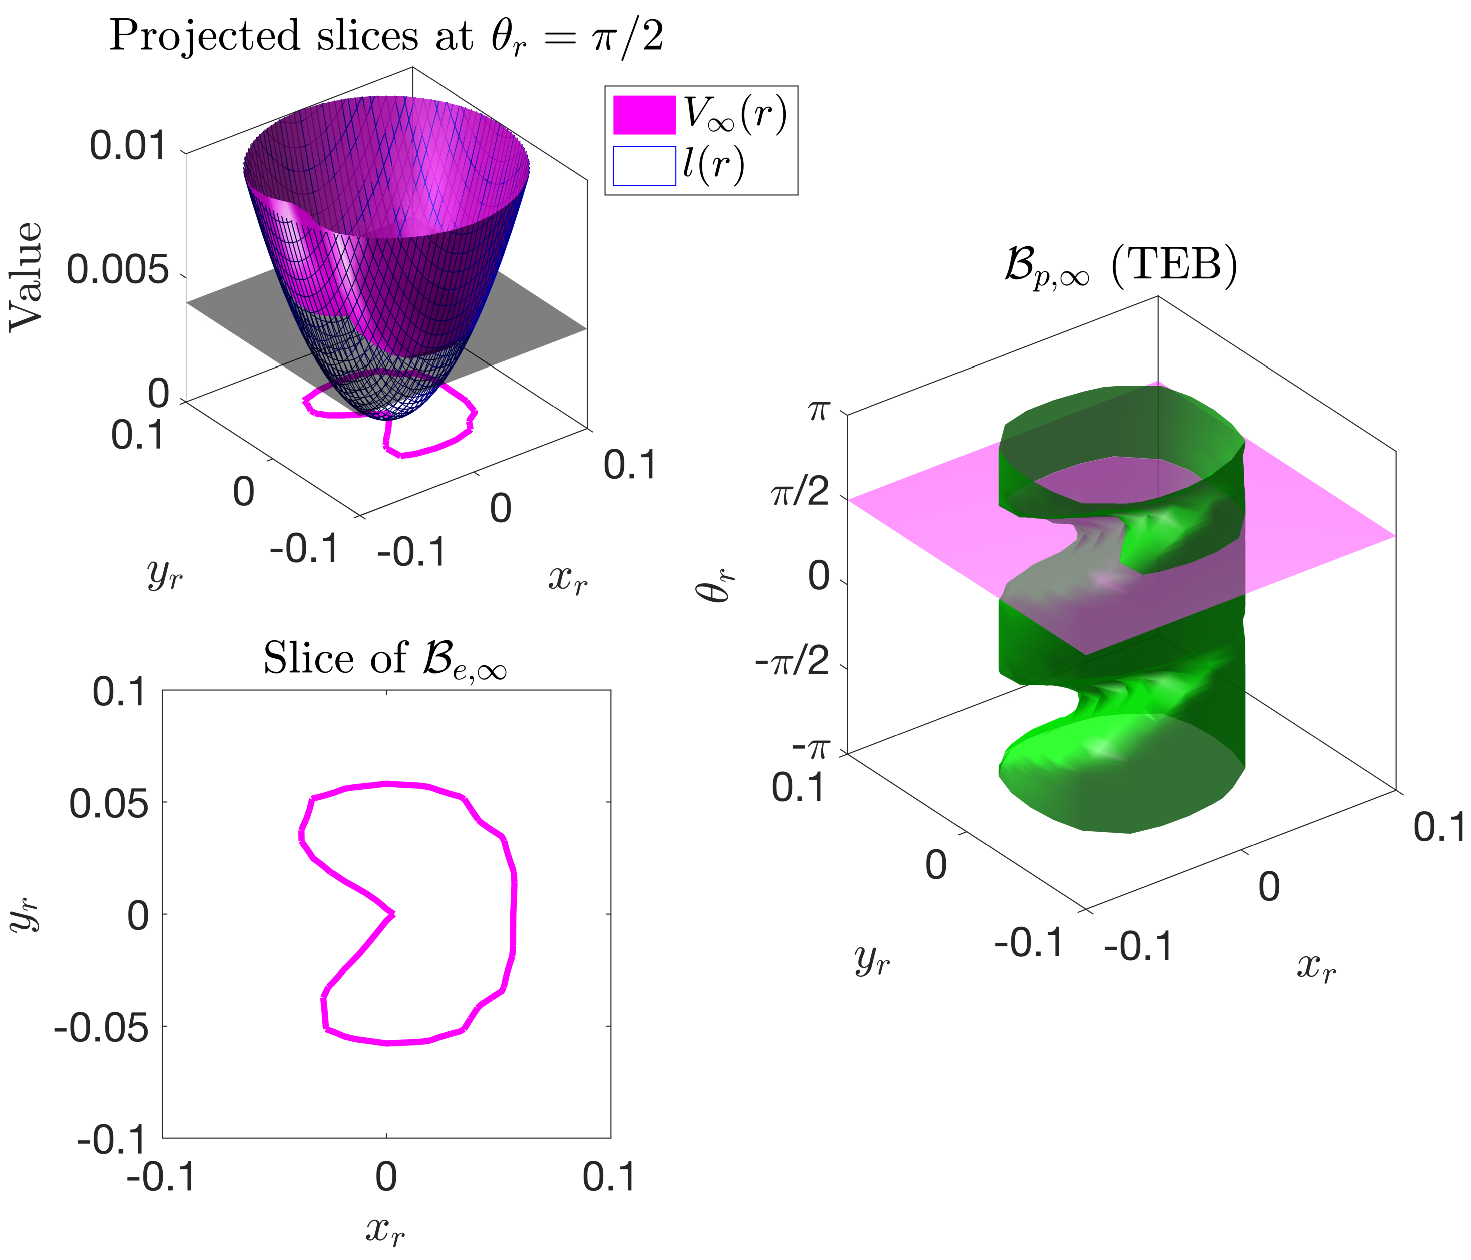
\includegraphics[width=\columnwidth]{fig/valfunc_illustration}
	\caption{Value function and TEB for the running example in \eqref{eq:5D_and_3D_err_state} and \eqref{eq:5D_and_3D_rdyn}. Top Left: projected slice ($\theta_r = \pi/2$) of the error function (blue hatch) and converged value function (magenta). The minimum value $\underline\valfunc$ of the converged value function is marked by the black plane; the slice of the value function at $\underline\valfunc$ determines the TEB (pink set), also shown on the bottom left.
		%. Bottom Left: closeup of this TEB (also projected at $\theta_r = \pi/2$) that corresponds to the minimum value $\underline\valfunc$ of the converged value function.  
		Right: the full TEB (no longer projected) in the error states. Note that the slice shown on the bottom right corresponds to the slice marked by the magenta plane at $\theta_r = \pi/2$.}
	\label{fig:valfunc_illustration}  
\end{figure}

\begin{figure}
	\centering
	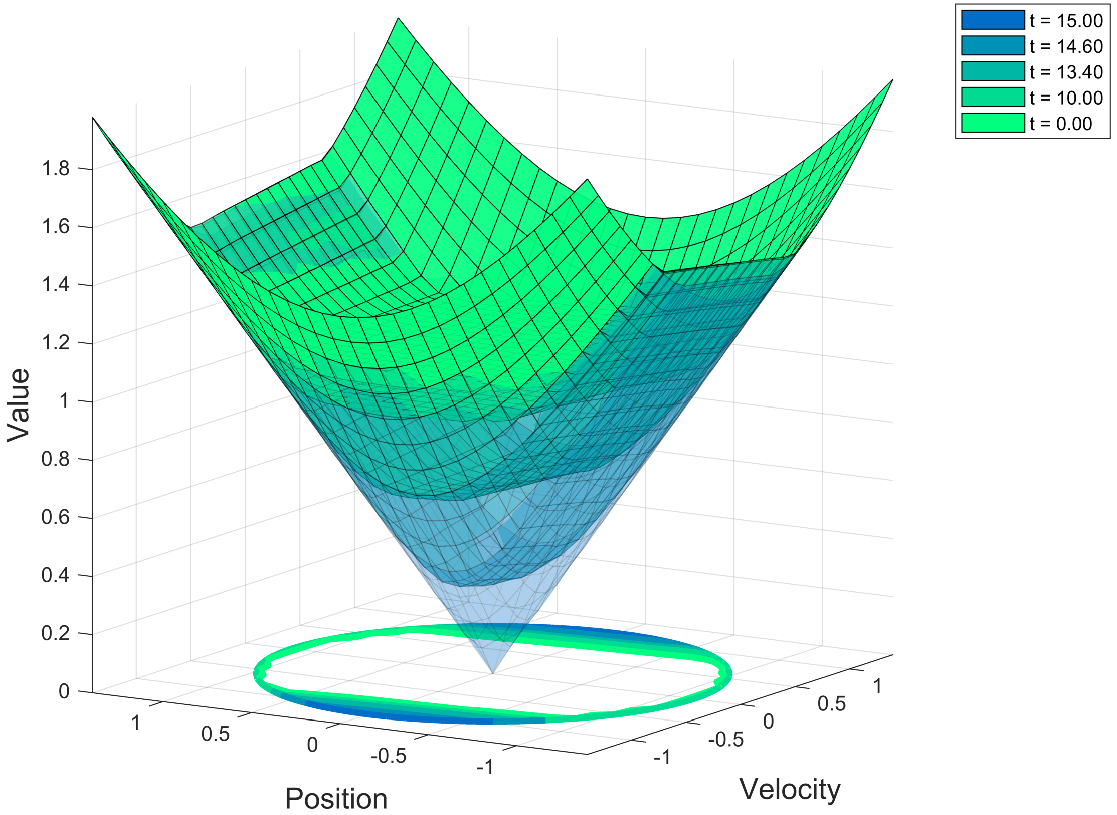
\includegraphics[width=\columnwidth]{fig/tv_valfunc}
	\caption{Time-varying value function (left) and TEBs (right) for the 8D quadrotor tracking 4D double integrator example in Section \ref{sec:resultsMPC}. The value function and the TEB varies with $\tau$, which represents time into the future. 
  The size of the TEB increase with $\tau$ because the disturbance and planning control may drive the error states farther and farther from the origin over time. 
  The error states shown are the relative position $x_r$ and velocity $v_{x,r}$.  Note that $\valfunc(\rstate,0) = \errfunc(\rstate)$.}
	\label{fig:vf_TEB:8D4D}
\end{figure} 

\begin{align}
\max \Big\{&\frac{\partial \tilde\valfunc}{\partial \tvar} + \min_{\tctrl\in\tset} \max_{\pctrl\in\pset, \dstb\in\dset} \nabla \tilde\valfunc \cdot \rdyn(\rstate, \tctrl, \pctrl, \dstb), \nonumber \\
&\qquad\errfunc(\rstate) - \tilde\valfunc(\rstate, \tvar)\Big\} = 0, \quad \tvar \in [-T, 0], \label{eq:HJVI} \\
&\tilde\valfunc(\rstate, 0) = \errfunc(\rstate), \nonumber
\end{align}

\noindent from which we obtain the value function, $\valfunc(\rstate, t) = \tilde\valfunc(\rstate, -t)$. There are many methods for solving this HJ VI; in this paper we focus on using the level set method toolbox \cite{Mitchell07c}.

If the planning model is ``close" to the tracking model and/or if the control authority of the tracking model is powerful enough to always eventually remain within some distance from the planning model, this value function will converge to an invariant solution for all time, i.e. $\valfunc_\infty(\rstate) := \lim_{\thor\rightarrow\infty} \valfunc(\rstate, \thor)$. 
Because the planning model is user-defined, convergence can often be achieved by tuning the planning model.

However, there may be tracking-planning model pairs for which the value function does not converge.  
In these cases the value function provides a finite time horizon, time-varying TEB, an example of which is shown in Fig. \ref{fig:vf_TEB:8D4D}.
Thus, even when convergence does not occur we can still provide time-varying safety guarantees.
In the rest of this paper, we will focus on the more general time-varying TEB case for clarity, and leave discussion of the time-invariant TEB case in the Appendix.
Our numerical examples will demonstrate both cases.

\example{In our running example we will set the cost to $\errfunc(\rstate) = x_r^2 + y_r ^2$, i.e. squared distance to the origin in position space. This means we only care about the autonomous system staying within an $(x_r,y_r)$ bound relative to the planning algorithm, and do not care about, for example, difference in relative angle.  We initialize equation (\ref{eq:HJVI}) with this cost function and the relative \ref{eq:5D_and_3D_rdyn}.  We propagate the HJ VI using the level set method toolbox until convergence or until we reach the planning horizon. In this case the value function converges to $\valfunc_\infty$ as seen in Fig. \ref{fig:vf_TEB:5D3D}. 
}

In Section \ref{sec:proofs}, we formally prove that sublevel sets of $\valfunc(\rstate,\tvar)$ provide the corresponding time-varying TEBs $\TEB(t)$ for the finite time horizon case.
The analogous result for the time-invariant, infinite time horizon case is proven in the appendix.

The optimal tracking controller is obtained from the value function's spatial gradient \cite{Mitchell05, Fisac15, Chen2018}, $\deriv(\rstate, \tvar)$, as

\begin{align} \label{eq:opt_ctrl_fin}
\tctrl^*(\rstate, \tvar) = \arg\min_{\tctrl\in\tcset} \max_{\pctrl\in\pcset, \dstb\in\dset} \nabla\valfunc(\rstate, \tvar) \cdot \rdyn(\rstate,\tctrl,\pctrl,\dstb)
\end{align}

To ensure the relative system remains within the TEB, we also note that the optimal (worst-case) planning control $\pctrl^*$ and disturbance $\dstb^*$ can also obtained from $\deriv(\rstate, \tvar)$ as follows:

\begin{align} \label{eq:opt_dstb_fin}
\begin{bmatrix}
  \pctrl^* \\
  \dstb^*
\end{bmatrix} (\rstate, \tvar) = \arg \max_{\pctrl\in\pcset, \dstb\in\dset} \nabla\valfunc(\rstate, \tvar) \cdot \rdyn(\rstate,\tctrl^*,\pctrl,\dstb)
\end{align}

For system dynamics affine in the tracking control, planning control, and disturbance, the optimizations in \eqref{eq:opt_ctrl_fin} and \eqref{eq:opt_dstb_fin} are given analytically, and provide the optimal solution to \eqref{eq:valfunc}.
In practice, the gradient $\deriv$ is saved as look-up tables over a grid representing the state space of the relative system.

\subsection{Error Bound Guarantee via Value Function} \label{sec:proofs}
We state the main theoretical result of this paper\footnote{The analogous infinite time horizon case is discussed in Prop. \ref{prop:main} in the Appendix.} in Prop. \ref{prop:nonconv}, which asserts that every level set of $\valfunc(\rstate, \tvar)$ is invariant under the following conditions:
\begin{enumerate}
  \item The tracking model applies the control in \eqref{eq:opt_ctrl_fin} which tries to track the planning model;
  \item The planning model applies the control in \eqref{eq:opt_dstb_fin} which tries to escape from the tracking model; \label{ln:plan}
  \item The tracking model experiences the worst-case disturbance in \eqref{eq:opt_dstb_fin} which tries to prevent successful tracking. \label{ln:dist}
\end{enumerate}

In practice, since the planning control and disturbance are \textit{a priori} unknown and are not directly controlled by the tracking model, conditions \ref{ln:plan} and \ref{ln:dist} may not hold. In this case, our theoretical results still hold; in fact, the absence of conditions \ref{ln:plan} and \ref{ln:dist} is advantageous to the tracking model and makes it ``easier'' to stay within its current level set of $\valfunc(\rstate, \tvar)$. 
The smallest level set corresponding to the value $\underline\valfunc := \min_{\rstate} \valfunc(\rstate,\thor)$ can be interpreted as the smallest possible tracking error of the system. 
The TEB is given by the set\footnote{In practice, since $\valfunc$ is obtained numerically, we set $\TEB(\tau) = \{\rstate: \valfunc(\rstate, \thor - \tau) \le \underline\valfunc + \epsilon\}$ for some suitably small $\epsilon>0$.}

\begin{align} \label{eq:TEB_fin}
\TEB(\tau) = \{\rstate: \valfunc(\rstate, \thor - \tau) \le \underline\valfunc\}.
\end{align}


Recall that we write the relative system state as $\rstate = (\estate, \astate)$, where $\estate,\astate$ are the error and auxiliary states.
Therefore, the TEB in the error state subspace is given by projecting away the auxiliary states $\astate$ in $\TEB(\tau)$:
  \begin{align} \label{eq:TEBp_fin}
  \TEB_\estate(\tau) = \{\estate: \exists \astate, \valfunc(\estate, \astate, \thor-\tau) \le \underline\valfunc\}
  \end{align}
  
This is the TEB that will be used in the online framework as shown in Fig. \ref{fig:fw_online}. 
Within this bound the tracking model may use any controller, but on the boundary\footnote{Practical issues arising from sampled data control can be handled using methods such as \cite{Mitchell2012, Mitchell13, Dabadie2014} and are not the focus of our paper.} of this bound the tracking model must use the optimal tracking controller.
In general, the TEB is defined as a set in the error space, which allows the TEB to not only be in terms of position, but any state of the planning model such as velocity, as demonstrated in the example in Section \ref{sec:resultsMPC}.

We now formally state and prove the proposition. 
Note that an interpretation of \eqref{eq:TEBp_fin} is that $\valfunc(\rstate, \thor - \tvar)$ is a control-Lyapunov function for the relative dynamics between the tracking model and the planning model.

\begin{prop}
  \label{prop:nonconv}
  \textbf{Finite time horizon guaranteed TEB.}
  Given $\tvar, \tvar' \in [0, \thor]$,
  
  \begin{subequations} \label{eq:fin_thor_prop}
      \begin{align}
      \forall \tvar' \ge \tvar, &~ \rstate \in \TEB(\tvar) \Rightarrow \rtraj^*(\tvar'; \rstate, \tvar) \in \TEB(\tvar'), \label{eq:fin_thor_prop:statement}\\
      \text{where} &\quad \rtraj^*(\tvar'; \rstate, \tvar) := \rtraj(\tvar'; \rstate, \tvar, \tctrl^*(\cdot), \pctrl^*(\cdot), \dstb^*(\cdot))), \label{eq:fin_thor_prop:here} \\
      &\quad
      \begin{aligned}
      &\tctrl^*(\cdot) = \arg \inf_{\tctrl(\cdot)\in\tcfset(t)}\big\{\\
      & \quad \max_{\tvar' \in [\tvar, \thor]} \errfunc(\rtraj(\tvar'; \rstate, \tvar, \tctrl(\cdot), \pctrl^*(\cdot), \dstb^*(\cdot))) \big\}, \label{eq:fin_thor_prop:ctrl}\\
      \end{aligned} \\
      &\quad
      \begin{aligned}
      & \pctrl^*(\cdot) := \gamma_\pstate^*[\tctrl](\cdot) = \arg \sup_{\gamma_{\pstate} \in \Gamma_\pstate(t)} \inf_{\tctrl(\cdot) \in \tcfset(\tvar)} \big\{ \\
      & \quad \max_{\tvar' \in [\tvar, \thor]} \errfunc(\rtraj(\tvar'; \rstate, \tvar, \tctrl(\cdot), \gamma_\pstate[\tctrl](\cdot), \dstb^*(\cdot))) \big\} \\
      \end{aligned} \\
      &\quad
      \begin{aligned}
      & \dstb^*(\cdot) = \arg \sup_{\gamma_{\dstb} \in \Gamma_\dstb(t)} \sup_{\gamma_{\pstate} \in \Gamma_\pstate(t)} \inf_{\tctrl(\cdot) \in \tcfset(t)} \big\{\\
      & \quad \max_{\tvar' \in [\tvar, \thor]} \errfunc(\rtraj(\tvar'; \rstate, \tvar, \tctrl(\cdot), \gamma_\pstate[\tctrl](\cdot), \gamma_\dstb[\tctrl](\cdot))) \big\}
      \end{aligned} \label{eq:fin_thor_prop:there}
      \end{align}
  \end{subequations}

\end{prop}

\begin{IEEEproof}
  
  We first show that given $\tvar, \tvar' \in [0, \thor]$,
  
  \begin{equation} \label{eq:vf_nondec}
    \forall \tvar' \ge \tvar, ~\valfunc(\rstate, \thor - \tvar) \ge \valfunc(\rtraj^*(\tvar'; \rstate, \tvar), \thor - \tvar')
  \end{equation}
  
  This follows from the definition of value function.
  \begin{subequations} \label{eq:fin_thor_steps}
    \begin{align}
      \valfunc(\rstate, \thor - \tvar) & = \max_{\tau \in [0, \thor-\tvar]} \errfunc(\rtraj^*(\tau; \rstate, 0)) \label{eq:fin_thor_steps:1} \\
      & = \max\{ \max_{\tau \in [0, \tvar'-\tvar]} \errfunc(\rtraj^*(\tau; \rstate, 0)), \nonumber\\
      &\qquad\qquad \max_{\tau \in [\tvar'-\tvar, \thor-\tvar]} \errfunc(\rtraj^*(\tau; \rstate, 0)) \} \label{eq:fin_thor_steps:2}\\
      & \ge \max_{\tau \in [\tvar'-\tvar, \thor-\tvar]} \errfunc(\rtraj^*(\tau; \rstate, 0)) \label{eq:fin_thor_steps:3}\\
      & = \max_{\tau \in [0, \thor-\tvar']} \errfunc(\rtraj^*(\tau; \rstate, \tvar-\tvar')) \label{eq:fin_thor_steps:4}\\
      & = \max_{\tau \in [0, \thor-\tvar']} \errfunc(\rtraj^*(\tau; \rtraj^*(0; \rstate, \tvar-\tvar'), 0)) \label{eq:fin_thor_steps:5}\\  
      & = \max_{\tau \in [0, \thor-\tvar']} \errfunc(\rtraj^*(\tau; \rtraj^*(\tvar'; \rstate, \tvar), 0)) \label{eq:fin_thor_steps:6}\\      
      & = \valfunc(\rtraj^*(\tvar'; \rstate, \tvar), \thor - \tvar') \label{eq:fin_thor_steps:7}
    \end{align}
  \end{subequations}

Explanation of steps:
\begin{itemize}
  \item \eqref{eq:fin_thor_steps:1} and \eqref{eq:fin_thor_steps:7}: by definition of value function, after shifting the time interval in \eqref{eq:fin_thor_prop:ctrl} to \eqref{eq:fin_thor_prop:there} from $[\tvar, \thor]$ to $[0, \thor-\tvar]$.
  \item \eqref{eq:fin_thor_steps:2}: rewriting $\max_{\tau \in [0, \thor-\tvar]}$ by splitting up the time interval $[0, \thor-\tvar]$ into $[0, \tvar'-\tvar]$ and $[\tvar'-\tvar, \thor-\tvar]$
  \item \eqref{eq:fin_thor_steps:3}: ignoring first argument of the outside $\max$ operator
  \item \eqref{eq:fin_thor_steps:4}: shifting time reference by $\tvar-\tvar'$, since dynamics are time-invariant
  \item \eqref{eq:fin_thor_steps:5}: splitting trajectory $\rtraj^*(\tau; \rstate, \tvar-\tvar')$ into two stages corresponding to time intervals $[\tvar-\tvar', 0]$ and $[0, \tau]$
  \item \eqref{eq:fin_thor_steps:6}: shifting time reference in $\rtraj^*(0; \rstate, \tvar-\tvar')$ by $\tvar'$, since dynamics are time-invariant
\end{itemize}

Now, we finish the proof as follows:
\begin{subequations} \label{eq:fin_hor}
  \begin{align}
  \rstate \in \TEB(\tvar) &\Leftrightarrow \valfunc(\rstate, \thor - \tvar) \le \underline\valfunc \\
  & \Rightarrow  \valfunc(\rtraj^*(\tvar'; \rstate, \tvar), \thor - \tvar') \le \underline\valfunc \label{eq:fin_hor:2}\\
  & \Leftrightarrow \rtraj^*(\tvar'; \rstate, \tvar) \in \TEB(\tvar'),
  \end{align}
\end{subequations}

\noindent where $\eqref{eq:vf_nondec}$ is used for the step in \eqref{eq:fin_hor:2}.

\end{IEEEproof} 

\begin{rem}
  As already mentioned, Prop. \ref{prop:nonconv} assumes that the planning control $\pctrl$ and disturbance $\dstb$ are optimally trying to maximize the value function $\valfunc$, and thereby increasing the size of the TEB $\TEB$.
  Despite this, \eqref{eq:fin_thor_prop:statement} still holds.
  In reality, $\pctrl$ and $\dstb$ do not behave in a worst-case fashion, and it is often the case that when $\tvar' \ge \tvar$, we have $\rstate \in \TEB(\tvar) \Rightarrow \rtraj(\tvar'; \rstate, \tvar) \in \TEB(\tau)$ for some $\tau \le \tvar'$.
  Thus, one can ``take advantage'' of the suboptimality of $\pctrl$ and $\dstb$ by finding the earliest $\tau$ such that $\rtraj(\tvar'; \rstate, \tvar) \in \TEB(\tau)$ in order to have the tighter TEB over a longer time-horizon.
\end{rem}

 \begin{rem} 
   Prop. \ref{prop:nonconv} is similar to well-known results in differential game theory with a slightly different cost function \cite{Akametalu2014}, and has been utilized in the context of using the subzero level set of $\valfunc$ or $\valfunc_\infty$ as a backward reachable set for tasks such as collision avoidance or reach-avoid games \cite{Mitchell05}. In this work we do not assign special meaning to any particular level set, and instead consider all level sets at the same time. This effectively allows us to effectively solve many simultaneous reachability problems in a single computation, thereby removing the need to check whether resulting invariant sets are empty, as was done in \cite{Bansal2017}.
 \end{rem}

\example{In our running example we have computed a converged value function $\valfunc_\infty$.  The corresponding TEB can be found using the converged form of (\ref{eq:TEB_fin}) found in the appendix as (\ref{eq:TEB_inf}). We can similarly find the TEB projected onto the planning states using (\ref{eq:TEBp_inf}). The minimum of the value function was approximately $\underline\valfunc = 0.004$, and the size of the TEB in $(x_r, y_r)$ space is approximately $0.065$. The converged value function and TEB can be seen in Fig. \ref{fig:vf_TEB:5D3D}. The corresponding optimal tracking controller is optained by plugging the gradients of our converged value function and our relative system dynamics into (\ref{eq:opt_ctrl_inf}). 
}